% !TEX root = main.tex

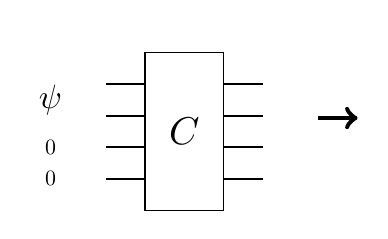
\begin{tikzpicture}


% \node[scale=1.25] at (-1.25,0.7){1)};
% \node[scale=1.4] at (-1,0){$\bigotimes_{i=1}^{n}\rho_i$};
% \node[scale=1.4] at (3.8,1/2+0.6){$A$};
% \node[scale=1.4] at (3.8,-1/2-0.6){$B$};
% \draw[line width=0.75] (0,0) -- (1,1/2+0.5);
% \draw[line width=0.75] (0,0) -- (1,1/2-0.4+0.5);
% \draw[line width=0.75] (0,0) -- (1,1/2+0.4+0.5);
% \draw[line width=0.75] (0,0) -- (1,1/2+0.8+0.5);


% \draw[line width=0.75] (0,0) -- (1,-1/2-0.5);
% \draw[line width=0.75] (0,0) -- (1,-1/2-0.4-0.5);
% \draw[line width=0.75] (0,0) -- (1,-1/2+0.4-0.5);
% \draw[line width=0.75] (0,0) -- (1,-1/2-0.8-0.5);

% \draw[line width=0.75] (3,1/2+0.5) -- (1,1/2+0.5);
% \draw[line width=0.75] (3,1/2-0.4+0.5) -- (1,1/2-0.4+0.5);
% \draw[line width=0.75] (3,1/2+0.4+0.5) -- (1,1/2+0.4+0.5);
% \draw[line width=0.75] (3,1/2+0.8+0.5) -- (1,1/2+0.8+0.5);

\draw[line width=0.75] (3,-1/2-0.5) -- (1,-1/2-0.5);
\draw[line width=0.75] (3,-1/2-0.5-0.4) -- (1,-1/2-0.4-0.5);
\draw[line width=0.75] (3,-1/2-0.5+0.4) -- (1,-1/2+0.4-0.5);
\draw[line width=0.75] (3,-1/2-0.5-0.8) -- (1,-1/2-0.8-0.5);



% \draw[line width=0.75] (3,1/2+0.5) -- (1,1/2-0.4+0.5);


% \node[draw, scale=1.25, fill=white] at (3.1,-1/2-0.4){$Z$};

% \node[draw, rounded rectangle west arc=none, scale=0.62, fill=white] at (1,-1/2-0.5+0.4){$I/X$};
% \node[draw, rounded rectangle west arc=none, scale=0.62, fill=white] at (1,-1/2-0.5){$I/X$};

\node[fill=white, scale=1.22] at (0.3,-1/2-0.5+1*0.2){$\ket{\psi}$};

% \node[fill=white, scale=0.79] at (0.3,-1/2-0.5+0.4){$\ket{0}$};
\node[fill=white, scale=0.79] at (0.3,-1/2-0.5-0.4){$\ket{0}$};
\node[fill=white, scale=0.79] at (0.3,-1/2-0.5-0.8){$\ket{0}$};
% \node[fill=white, scale=0.79] at (0.3,-1/2-0.5){$\ket{0}$};
% \node[scale=1.29] at (3.6,-1/2-0.45){$\ket{\psi}$};

% \node[draw, rounded rectangle, rounded rectangle west arc=none, scale=0.75, fill=white] at (3.1,-1/2-0.4-0.5){$Z$};
% \node[draw, rounded rectangle, rounded rectangle west arc=none, scale=0.75, fill=white] at (3.1,-1/2-0.5-0.8){$Z$};
    % \node [rounded rectangle east arc=none, below=of B]{};

% \draw[line width=1.25] (3,1/2) -- (1,1/2);
% \draw[line width=1.25] (0,0) -- (1,-1/2);
% \draw[line width=1.25] (3,-1/2) -- (1,-1/2);
% \node[draw, scale=1.5, fill=white] at (3,-1/2){$P$};
% \node[draw, scale=1.5, fill=white] at (2,-1/2){$C$};
% \node[draw, scale=1.25, fill=white] at (2.1,1/2){$C^{T}$};
% \draw[draw=black, fill=white] (1.5,1/2-0.3) rectangle ++(1.0,2.0) node[pos=.5, scale=1.4]{$C^T$};

\draw[draw=black, fill=white] (1.5,-1/2-0.3-1.4) rectangle ++(1.0,2.0) node[pos=.5, scale=1.4]{$C$};
% \node[draw, scale=1.25, fill=white] at (2.1,-1/2){$C^{\dagger}$};
\node[anchor=east] at (3.5, 0) (node1){};
\node[anchor=east] at (3.5, -1.25) (node2){};
% \draw[->, line width=0.3mm] (node1) to [out = -45, in = 45, looseness = 1] (node2);
\draw [->, line width=1.8pt](3.7,-1.03) -- (4.2,-1.03);

    % \draw [-stealth](2,-2.6) -- (2,-3.1);
\end{tikzpicture}